% \chapter{(占位)}
\chapter{需要了解的知识}

\begin{quote}
    亵慢的人受刑罚,愚蒙的人就得智慧。智慧人受训诲,便得知识。
    
    \hfill《圣经·箴言》12:11
\end{quote}


本章要研究使用\LaTeX 生成文档时的基本排版指令。我们将零散地处理用于突出显示、\LaTeX 标准环境、标题、页面下方的注释、页眉和页脚,以及浮动的环境。接下来,我们会介绍参考系统和\LaTeX 生成的辅助文件。最后,阅读到本章末尾的人将有机会读到一些关于断字的思考。

所有这些指令都将以其默认行为模式使用。也就是说,我们这里不介绍重新定义它们的方法。对应地,你将能够以传统的版式来生成文档。若要打出一篇更进阶的文章,你需要了解如何输入数学式(第3章)、一些关于科技文档的知识(第6章),以及包含图像的方法(第5章)。

\section{突出显示}

要了解\LaTeX 选用字体的机制,需要知道:我们通常通过4个参数来区别字体。

\begin{description}
  \item[族(famille)] 指字体的整体形状。默认情况下,\LaTeX 使用三种字体族:罗马体、\textsf{无衬线体}、\texttt{打字机体}。\LaTeX 中,以英文单词\emph{family}来指代字体族。
  \item[风格(style)] 指字体体现出的体态(英文以\emph{shape}指代),分为:\textit{意大利体}、\textsl{倾斜}和\textsc{小型大写字母风格(petites capitales)}\yz{
    本书翻译时,以楷体对应意大利体、以仿宋体对应倾斜排版,按原文翻译。中文字体的族和风格往往是并列的,很少有交叉叠加的情况,因此在展示叠加效果时酌情保留原文。中文中很少见到类似小型大写字母的突出显示方式。因此,除了特意展示西文的部分外,本书忽略小型大写字母格式,必要时以其他风格取代。
  }。
  \item [字重(graisse)]指字体笔画的粗细(\LaTeX 中以\emph{serie}指代)。默认情况下有两种粗细:中等和\textbf{加粗}。
  \item [字号]字{\large 体}{\Large 的}{\LARGE 大}{\small 小}。
\end{description}


\subsection{族--风格--字重}

有两种不同的宏可以设置族、风格、字重这三个变量:\emph{指令}和\emph{声明}(如表\ref{tab:2.1}所示)。指令以花括号的形式将其参数括住。声明可以打断行文,同时修改三个变量之一,直到新的命令出现。总体上的规则是,我们使用指令来突出显示一个词或一组词:

\begin{table}
    \centering
    \begin{tabular}{|c|l|c|}
\hline
指令 & 声明 & 输出\\
\hline
\verb+\textrm{...}+ & \verb+{\rmfamily ...}+ & 罗马(roman) \\
\verb+\textsf{...}+ & \verb+{\sffamily ...}+ & \textsf{非衬线(sans sérif)} \\
\verb+\texttt{...}+ & \verb+{\ttfamily ...}+ & \texttt{打字机(machine à écrire)} \\
\hline
\verb+\textup{...}+ & \verb+{\upshape ...}+ & 正(droit) \\
\verb+\textit{...}+ & \verb+{\itshape ...}+ & \textit{意大利(italique)} \\
\verb+\textsl{...}+ & \verb+{\slshape ...}+ & \textsl{倾斜(penché)} \\
\verb+\textsc{...}+ & \verb+{\scshape ...}+ & \textsc{小型大写(Petites Capitales)} \\
\hline
\verb+\textmd{...}+ & \verb+{\mdseries ...}+ & 中等(médium) \\
\verb+\textbf{...}+ & \verb+{\bfseries ...}+ & \textbf{加粗(gras)} \\
\hline
    \end{tabular}
    \caption{更改字体的声明}
    \label{tab:2.1}
\end{table}

\begin{codelist}[2.1]{
    \texttt{char}类型的\emph{变量}\textsl{总是}被编码为\textbf{8 位}。
}
\begin{verbatim}
\texttt{char}类型的\emph{变量}\textsl{总是}被编码为\textbf{8 位}。
\end{verbatim}
\end{codelist}

注意,在上面的命令中,指令\verb|\emph|(对应的声明是\verb|\em|,可以以更优雅的方式突出显示一组词)。相较声明,强烈建议使用\emph{指令}。当要修改文本的一部分时,使用指令是更明智的选择\jz{定义指令也是。}:

\begin{codelist}[2.2]{
    {\em \bfseries 马格马(Magma) \mdseries 的音乐就像一面镜子,每个人都能看到他自己的倒影。}
}
    \begin{verbatim}
{\em \bfseries 马格马(Magma) \mdseries 的音乐
就像一面镜子,每个人都能看到他自己的倒影。}
    \end{verbatim}
\end{codelist}

接下来的例子展示了如何使用组。声明\verb|\slshape|出现在一个组中,因此它只在组内发挥作用。此外,组会继承它外层的组的参数。这样一来,“silence”一词会使用\textsf{非衬线}体(根据外层的组),并且\textsl{倾斜}展示(根据内层的声明):

\begin{codelist}[2.3]{
    \sffamily 在爵士乐中,{\slshape 沉默(silence)\/}永远是正确的。因此,这是一种充满万千可能的音乐。
}\begin{verbatim}\sffamily 在爵士乐中,
{\slshape 沉默(silence)\/}永远是正确的。因此,
这是一种充满万千可能的音乐。
\end{verbatim}
\end{codelist}

\subsection{意大利体校正}

另一个推荐使用指令而不是声明的理由是,与声明不同,指令可以实现\emph{意大利体校正}。所谓意大利体校正,是指在以意大利体显示的字符组后,有必要增加一个间距,使得这组字符不会“碰到”后面的词。这个间距与所涉及的字符有关\yz{此例展示不同情况下\emph{f}和a间距的细微差距,宜保留原文。例句意为:首长永远是对的。}:

\begin{codelist}[2.4]{
    le {\em chef} a toujours raison.\par
    le {\em chef\/} a toujours raison.\par
    le \emph{chef} a toujours raison.\par
}\begin{verbatim}le {\em chef} a toujours raison.\par
le {\em chef\/} a toujours raison.\par
le \emph{chef} a toujours raison.\par
\end{verbatim}
\end{codelist}

我们可以看到,指令\verb|\emph|实现了校正,然而,若要使用声明,则需要明确地借助宏\verb|\/|来实现相同的效果。

\subsection{字号}

表\ref{tab:2.2}中展示的宏可以修改行文的字号。这些宏都是\emph{声明}。同时,对于每一个宏都存在同名的环境。

\begin{table}[ht]
    \centering
    \begin{tabular}{|c|c||l|c|}
\hline
\verb|\Huge| & {\Huge 宏大} & \verb|\normalsize| & {正常} \\
\verb|\huge| & {\huge 庞大} & \verb|\small| & {\small 小} \\
\verb|\LARGE| & {\LARGE 特大} & \verb|\footnotesize| & {\footnotesize 加小} \\
\verb|\Large| & {\Large 加大} & \verb|\scriptsize| & {\scriptsize 特小} \\
\verb|\large| & {\large 大} & \verb|\tiny| & {\tiny 微小} \\
\hline
    \end{tabular}
    \caption{修改字号}
    \label{tab:2.2}
\end{table}

\subsection{几个建议}

习惯上,我们应当尽量减少字体变化。实际上,如果字体变化得不合适宜或没有实际用处,尤其是喧宾夺主,影响了文档的可读性,看起来就会很低级。这里是有关使用字体变化的几条建议(仍然是习惯上的建议!):
\begin{itemize}
    \item 相较于使用其余指令,更多地使用\verb+\emph+(默认会将字体改为\emph{意大利}体)。
    \item 将\textbf{加粗}的机会留给特别重要的提示。
    \item 在法文文档中,几乎只在人名中使用小型大写字母(如Donald \textsc{Knuth})。
    \item \dm{打字机}字体族经常被用于生成编程语言的代码或类似的内容。
\end{itemize}

以下内容适用于能读懂其中道理的人……

除以上内容外,我们给出以下两个用于突出显示的情况,读者可以字形斟酌:改变字号、添加下划线(使用指令\verb|\underline|)。

\begin{quote}
    也许那些希望{\tiny 小声说话}的诗人会让图书的字体频繁变化,但目前,只有一些字体狂人{\tiny (比如本手册的作者)}才喜欢这样做。
    
    \hfill 克努特,\TeX Book[9]
\end{quote}

\begin{quote}
    注意,出版行业认为,以添加下划线的形式来强调内容是不好的习惯。下划线只应用于一种情况——输出设备无法以其他方式突出显示内容,比如使用打字机。
    
    \hfill 迈克尔·古森斯(Michel Goossens)等,《\LaTeX 伴侣》(\emph{\LaTeX{} Companion})[6]
\end{quote}

\section{环境}

\LaTeX 以\emph{环境}格式提供了一系列工具,具体结构是一个代码块,语法如下:

\begin{dmd}
    \verb+\begin+\codereplace{环境名}\verb|}|\\
    \verb|...|\\
    \verb+\end+\codereplace{环境名}\verb|}|\\
\end{dmd}

其中\codereplace{环境名}需要替换为具体的环境名称。我们目前遇到的第一个环境是\dm{document}。\verb|\begin| 和\verb|end|间的文字会以特殊版式展示。

\begin{exclamation}
    我们立刻注意到,环境中所有声明都是局部的。另外,当然可以在我们自己定义的环境中套用已经存在的环境。
\end{exclamation}

\subsection{居中和对齐}

想要居中显示几行文字,我们使用环境\dm{center}:

\begin{codelist}[2.5]{
    ……上一段的结尾。
    \begin{center}
        完美居中的\\
        几行文字\\
        且前后带有间距
    \end{center}
    然后继续下一段……
}\begin{verbatim}……上一段的结尾。
\begin{center}
  完美居中的\\
  几行文字\\
  且前后带有间距
\end{center}
然后继续下一段……
\end{verbatim}
\end{codelist}

同样,我们可以轻易地借助环境\dm{flushright},让一个段落右对齐排列:

\begin{codelist}[2.6]{
    ……上一段的结尾。
    \begin{flushright}
      两行右对齐\\
      的文字
    \end{flushright}
    然后继续下一段……
    }{
\begin{verbatim}……上一段的结尾。
\begin{flushright}
  两行右对齐\\
  的文字
\end{flushright}
然后继续下一段……
\end{verbatim}
    }
\end{codelist}

注意,以上两个示例中,命令\verb|\\|起到了换行的功能。除一些特殊场景(表格、文档的标题和作者、特意的居中或对齐处理)外,不要使用这个命令——如果想要换行,需要使用空行或命令\verb|\par|。

\begin{flushleft}
    一般情况下,我们使用环境\dm{flushleft}时需要搭配命令\verb|\\|。但我们可以使用这个环境来生成右侧不对齐的文档,将换行的麻烦工作留给\LaTeX ,就像这段文字一样。(译注:此处给出本段原文。请注意右侧的换行的不对齐处理。En général, on emploie l'environnement \dm{flushleft} avec des commandes \verb|\\|. Mais on peut l'utiliser pour produire un paragraphe comme celui-ci, non justifié à droite, en laissant à \LaTeX{} le soin d’insérer les sauts de lignes.)
\end{flushleft}

%TODO 排查代码下正文内容
\begin{exclamation}
    绝大部分环境都会重启一行来插入内容。然而,重要的是:环境只是在插入内容的位置\emph{中断}当前段落,而不是结束当前段落。你可以在前两个实例中看到,“然后继续下一段……”这句话前没有缩进。另外,\LaTeX 贴心地在每个环境前后都留了一段空白。
\end{exclamation}

我们可以注意到,前面的三个环境分别代表以下三个声明:

\begin{itemize}
    \item \verb|\centering|;
    \item \verb|\raggedleft|;
    \item \verb|\raggedright|。
\end{itemize}

例如,我们可以这样写\yz{
    实际上,Emacs代表Editor MACroS。本例是对Emacs的调侃。
}:

\begin{codelist}[2.7]{
    Emacs代表:

    {\centering Emacs\\Makes\\
      A\\Computer\\Slow\\}
}{\begin{verbatim}Emacs代表:

{\centering Emacs\\Makes\\
  A\\Computer\\Slow\\}
\end{verbatim}
}
\end{codelist}

\subsection{列表}

\LaTeX 提供了三种呈现\emph{列表}的基本环境:\dm{itemize}、\dm{enumerate}、\dm{description}。如果它们都不能满足你,也可以定义属于你自己的\celan{9.5节}列表。但目前,先来看看标准的列表。

首先,\dm{itemize}可以生成不编号的项目列表。在法文版本中,一级列表会使用连接号(---)标记;在其他版本中,会使用点($\bullet$)标记:

\begin{codelist}[2.8]{
……一句话的结尾。
\begin{itemize}
\item 在复杂的计算中,分子的系数需要传递给分母;
\item 不应当写逗号。
\end{itemize}
然后行文继续。
}\begin{verbatim}
……一句话的结尾。
\begin{itemize}
\item 在复杂的计算中,
  分子的系数需要
  传递给分母;
\item 不应当写逗号。
\end{itemize}
然后行文继续。
\end{verbatim}
\end{codelist}

环境\dm{enumerate}遵循类似的规则,只不过项目会被编号。一个环境中可以套用另一个环境。下面的例子中,我们同时展示了\dm{ enumerate}和\dm{description}环境:

\begin{codelist}[2.9]{
    ……还是一句话的结尾。
    \begin{description}
    \item[\TeX] \TeX{}book;
    \item[\LaTeX] 两本重要的书:
      \begin{enumerate}
      \item 《\LaTeX{}:一个文档准备系统》(\emph{\LaTeX{}: A Document Preparation System})。
      \item 《\LaTeX{}伴侣》。
      \end{enumerate}
    \end{description}
    跟之前一样,接下来段落继续……
}\begin{verbatim}……还是一句话的结尾。
\begin{description}
\item[\TeX] \TeX{}book;
\item[\LaTeX] 两本重要的书:
  \begin{enumerate}
  \item 《\LaTeX{}:一个文档
    准备系统》(\emph{\LaTeX{}: 
    A Document Preparation System})。
  \item 《\LaTeX{}伴侣》。
  \end{enumerate}
\end{description}
跟之前一样,接下来段落继续……
\end{verbatim}
\end{codelist}

至于环境\dm{description}的列表,在我们习惯的文档处理中没有对应内容。不幸的是,对于\LaTeX 初学者,它最好的结果是被误用,最差的结果是被无视。

\subsection{制表}

环境\dm{tabbing}可以用于打字机上使用的那种老式制表过程%TODO查证
。我们可以使用指令\verb|\=|来放置定位标记,并使用指令\verb|\>|来在定位标记之间移动。此外,\verb|\\|可以用来换行。

\begin{codelist}[2.10]{
  \begin{tabbing}
    左倾 \= 中间立场 \= 右倾 \\
    \> 中立派 \\
    \> \> 保守派 \\
    xxxxxxxxx \= \kill
    \> 无观点
    \end{tabbing}
}\begin{verbatim}
\begin{tabbing}
  左倾 \= 中间立场 \= 右倾 \\
  \> 中立派 \\
  \> \> 保守派 \\
  字字字字字 \= \kill
  \> 无观点
\end{tabbing}
\end{verbatim}
\end{codelist}

我们可以从这个例子中看到两个规则:

\begin{itemize}
    \item 可以在制表时插入一行“模板”,并且使用指令\verb|\kill|来隐藏这一行;
    \item 如果已经存在定位标记,新的指令\verb|\=|可以在逻辑上移除它们。
\end{itemize}

\subsection{表格}

\LaTeX 中用于生成\emph{表格}的环境称为\dm{tabular}。表线的处理可能不太精细,但对于线条简单的表格,结果可以接受\jz{
    附录B提供了一些提示,可以用来找到能够生成更复杂表格的包。
}:

\begin{codelist}[2.11]{
    嚯:
    \begin{tabular}{|r|c|}
        \hline
        俩 & 仨 \\
        五个 & 六个  \\ \hline
      \end{tabular}
}\begin{verbatim}嚯:
\begin{tabular}{|r|c|}
  \hline
  俩 & 仨 \\
  五个 & 六个  \\ \hline
\end{tabular}
\end{verbatim}
\end{codelist}
通过这个例子,我们可以得到以下结论。

\begin{itemize}
    \item 环境\dm{tabular}会等待输入一个参数,应用指示表格的格式。每列都应该以一个定位字符表示。
    \begin{itemize}
        \item \dm{r}:右对齐。
        \item \dm{c}:居中。
        \item \dm{l}:左对齐。
    \end{itemize}
    \item 字符\verb|&|用于分隔不同列。
    \item 指令\verb|\\|用于跳转至下一行。
    \item 布局字符串中的\dm{|}表示插入纵向表线。
    \item 横向表线由指令\verb|\hline|插入。
\end{itemize}

因此,我们可以自由地调整\verb|\hline|和\dm{|}的数量,以隐藏或显示表线。包\textsf{array}可以满足一些关于表格的幻想。

\begin{exclamation}
大多数环境都会另起一行,但\dm{tabular}不会。\dm{tabular}会紧接当前的文本生成表格。
\end{exclamation}

此外,我们还可以使用参数来精确地指定表格竖直方向上的位置:

\begin{codelist}[2.12]{
一个表:\begin{tabular}[b]{|c|} 
甲\\乙
\end{tabular}
,另一个表:\begin{tabular}[t]{|c|} 
丙\\丁\end{tabular}
}\begin{verbatim}一个表:\begin{tabular}[b]{|c|} 
  甲\\乙
\end{tabular}
,另一个表:\begin{tabular}[t]{|c|} 
  丙\\丁
\end{tabular}
\end{verbatim}
\end{codelist}

我们可以看出,参数\dm{b}将表格“放置”在当前行上,参数\dm{t}将表格“悬挂”在当前行下。如果没有参数,表格会在竖直方向上居中,就像前面的例子一样。

显然,表格可以不插入句子中,而可以单独成段,比如配合环境\dm{center}被单独居中。

\subsection{模拟终端}

环境\dm{verbatim}可以将其内容逐字插入文档。因此,无论什么字符,甚至是特殊字符,都可以使用它来插入,如插入一个\textsf{C++}代码片段:

\begin{codelist}[2.13]{\ttfamily
  \begin{tabbing}
    cl\=ass pixel \{\\
      \>int x, y;\\
    public:\\
      \>pixel(int i=0, int j=0);\};
  \end{tabbing}
}
\ttfamily
\backslash begin\{verbatim\}
\begin{verbatim}
class pixel{
  int x,y;
public:
  pixel(int i=0, int j=0);};
\end{verbatim}
\backslash end\{verbatim\}
\end{codelist}

\begin{exclamation}
我们可以在环境\dm{verbatim}中写任何内容,\emph{除了}以下字符串——\verb|\end{verbatim}|!
\end{exclamation}

有两个指令可以像\dm{verbatim}一样生成文本片段:\verb|\verb|和\verb|\verb*|。带有星号的版本可以将空格“\verb| |”显示为“\verb*| |”的形式。

这两个指令的参数不使用花括号括起,而夹在任何一种可以满足以下两个条件的符号之间:不能是特殊符号、不能在参数中包含:

\begin{codelist}[2.14]{
  使用{\ttfamily \#include<stdlib.h>+}可以
  包含C语言标准库的原型。
}\begin{verbatim}
使用\verb+#include<stdlib.h>+可以
包含C语言标准库的原型。
\end{verbatim}
\end{codelist}

\begin{exclamation}
在任何情况下,指令\verb|\verb|都不能出现在其他指令的参数中,无论这个指令是什么。
\end{exclamation}

\subsection{引用语}

环境\dm{quote}和\dm{quotation}可以在文本中引用内容。首先来看\dm{quote}:

\begin{codelist}[2.15]{
  ……仍然是一句话的结尾。
\begin{quote}
  万物相关。\hfill\textbf{爱因斯坦}

  有件事情是不确定的,
  那就是所有事情都是确定的。
  \hfill\textbf{帕斯卡}
\end{quote}
然后继续被打断的段落……
}\begin{verbatim}
……仍然是一句话的结尾。
\begin{quote}
  万物相关。\hfill\textbf{爱因斯坦}

  有件事情是不确定的,
  那就是所有事情都是确定的。
  \hfill\textbf{帕斯卡}
\end{quote}
然后继续被打断的段落……
\end{verbatim}
\end{codelist}

指令\verb|\hfill|可以插入一段在水平空间上\celan{\S 4.2.4}无限延伸的空白。环境\dm{quotation}有一些细微的差别:

\begin{codelist}[2.16]{
  ……仍然是一句话的结尾。
\begin{quotation}
  人有许多缺陷,但我们若能
  想到他们被创造的那个年代,
  就能对此感到宽容。\par
  \raggedleft 阿方斯·阿莱
  (Alphonse Allais)
\end{quotation}
然后继续被打断的段落……
}\begin{verbatim}
……仍然是一句话的结尾。
\begin{quotation}
  人有许多缺陷,但我们若能
  想到他们被创造的那个年代,
  就能对此感到宽容。\par
  \raggedleft 阿方斯·阿莱
  (Alphonse Allais)
\end{quotation}
然后继续被打断的段落……
\end{verbatim}
\end{codelist}

实际上,对于这两个环境,根据莱斯利·兰波特的介绍,一个(\dm{quote})是为引用一条或多条短的内容而准备的,另一个(\dm{quotation})是为引用一条长的内容而准备。

\section{页边注}

指令\verb|\marginpar|可以在页边缘创建一个小段落,语法如下:

\begin{dmd}
\backslash marginpar\{\codereplace{文字}\}
\end{dmd}

对于双面打印的模式,为了区分左侧和右侧的页面,我们可以使用如下指令\yz{
  原书有误。此处已更正。
}:

\begin{dmd}
\backslash marginpar[\codereplace{左侧文字}]\{\codereplace{右侧文字}\}
\end{dmd}

其中\codereplace{左侧文字}和\codereplace{右侧文字}会根据当前页码的奇偶性在页面左侧或右侧呈现。如此一来,以下指令:

\begin{dmd}
\backslash marginpar[这!]\{嚯!\}
\end{dmd}\marginpar[这!]{嚯!}

会生成你在本页页边缘看到的内容。

\section{标题}

表\ref{tab:2.3}给出了\LaTeX 种可用的\emph{章节}命令。对于类型为\dm{article}的文档,指令\verb|\chapter|不可用;对于类型为\dm{letter}的文档,任何标题类型都不可用。目前,你需要了解以下两点:

\begin{itemize}
  \item 使用指令生成的每个标题都可以自动\emph{编号},并可以在必要时列入目录。
  \item 使用指令\verb|\tableofcontents|可以生成目录,并将其插入该指令所在的位置。
\end{itemize}

\begin{table}[ht]
  \centering
  \begin{tabular}{|l|l|l|}
    \hline
    \verb|\part{...}| & \verb|\chapter{...}| & \\
    \verb|\section{...}| & \verb|\subsection{...}| & \verb|\subsubsection{...}| \\
    \verb|\paragraph{...}| & \verb|\subparagraph{...}| &  \\
    \hline
  \end{tabular}
  \caption{章节指令}
  \label{tab:2.3}
\end{table}

\begin{ii}
此外,所有的标题指令都带有可以自定义的相关类型。% TODO
总的来说,这些指令会自动生成标题前后的间距。如此一来,指令前后的任何空行都会被忽略。
\end{ii}

\begin{codelist}[2.17]{
  ……一句话的结尾。
  \section*{3.2\quad 结论}
  最终,……
}\begin{verbatim}
……一句话的结尾。
\section{结论}
最终,……
\end{verbatim}
\end{codelist}

每种标题指令都带有一种“带星”形式(例如,\verb|\section*|),可以插入不参与编号的标题。但需要注意,这种标题不会出现在\celan{\S 2.9.2}目录中。与节(section)相关的标题指令中可以接受参数,用于明确目录中展示的内容。例如:

\begin{dmd}
\verb+\section[张三]{太帅了!}+
\end{dmd}

可以在文档中插入节标题“太帅了!”,但在目录中将其展示为“张三”。

\section{页面底部的注释}

有一种方便的方式可以在页面底部插入注释:使用指令\verb|\footnote{|\codereplace{文本}\verb|}|。注释会自动编号,且在默认情况下按章重新编号。如下是\LaTeX 可以实现的效果:

\begin{codelist}[2.18]{
  无论如何,指令\texttt{footnote}$^a$可以在页面底部插入注释。\\
  ————\\%TODO 
  {\footnotesize $^a$正如其名。}
}\ttfamily
无论如何,指令\backslash verb +footnote+
\backslash footnote\{正如其名。\}可以在页面
底部插入注释。\rmfamily
\end{codelist}

在一些特殊情况中,\verb|\footnote|不能生成我们想要的效果。此时,有必要分两步走:

\begin{enumerate}
  \item 使用指令\verb|\footnotemark|放置\emph{注释标记};
  \item 当条件允许时,使用指令\verb|\footnotetext|在页面底部输入\emph{文字}。
\end{enumerate}

例如,在表格中插入注释似乎有点棘手,此时可以这样写:

\begin{codelist}[2.19]{
  \begin{tabular}{cc}
    甲 & 乙$^a$ \\
    丙 & 丁\\
  \end{tabular}\\
  ————\\
  {\footnotesize $^a$一个注释。}
}\begin{verbatim}
\begin{tabular}{cc}
  甲 & 乙\footnotemark \\
  丙 & 丁
\end{tabular}\footnotetext{一个注释。}
\end{verbatim}
\end{codelist}

\section{页眉和页脚}

\LaTeX 生成页眉和页脚的标准指令有些简陋,但这里也值得一提,因为这些指令对于一些特定情况已经足够了。

\begin{ii}
关于这些指令,在这里就不讲更多内容了,因为\dm{fancyhdr.dvi}中介绍的fancyhdr包易用得多,也提供了比\LaTeX 的标准指令多得多的有趣选项。本书关于使用此包生成页眉页脚的详细解释在10.4节。
\end{ii}

如果不调用其他包,可以在文档的文前部分使用指令\verb|\pagestyle|来指定页眉页脚的风格:

\begin{dmd}
\verb|\pagestyle{|\codereplace{风格}\verb|}|
\end{dmd}

其中,参数\codereplace{风格}可以从以下值中选择:

\begin{itemize}
  \item \dm{empty},不显示页眉和页脚;
  \item \dm{plain},默认风格,页脚居中显示当前页码;
  \item \dm{headings},在页眉显示一定的内容,根据文档风格的不同而不同(例如,在双面的\dm{report}文档中,会显示当前的章名或节名);
  \item \dm{myheadings},自定义插入内容。
\end{itemize}

此外,使用指令\verb|\thispagestyle|,可以变更或指定当前页的风格。

\section{浮动环境}

\LaTeX 为其优秀的用户提供了使用\emph{浮动}环境的可能性。这种环境的特点是,其内容会被“漂浮地”渲染到正文中。也就是说,\LaTeX 通过一种算法,综合考虑一系列参数,在文档中为这种环境挑选位置。

\begin{exclamation}
\LaTeX 中的环境\dm{figure}和\dm{table}并不仅仅可以用来插入图片和表格,这一点与它们的名字相反。实际上,这两种环境只是将其内容浮动起来,并且为添加图题或表题提供了可能性。实际上,这两种环境中可以是你喜欢的任何内容,也不一定要是图形。
\end{exclamation}

\subsection{图(figure)和表(table)}

环境\dm{figure}一般用来插入图像,而环境\dm{tale}一般用于插入表格。这两种环境都可以带有自己的小标题,使用语法如下:

\begin{codelist}[2.20]{
  此段包含了浮动环境“figure”,
其内容可以在页面中浮动。
% \begin{figure} 插环境会报错
  \begin{center}
三\\
O丁O\\
四\\
Figure 1: 有个老丁头
  \end{center}
%   \caption*{有个老丁头}
% \end{figure}

}\begin{verbatim}
此段包含了浮动环境“figure”,
其内容可以在页面中浮动。
\begin{figure}
  \begin{center}
    三\\
    O丁O\\
    四\\
  \end{center}
  \caption{有个老丁头}
\end{figure}
\end{verbatim}
\end{codelist}

注意到,使用指令\verb|\caption|可以生成图题或表题。文本“Figure 1:”会自动生成,并给出对应该图片的编号。这种“风格”也是可以自定义的。

\subsection{确定位置}

我们可以在\verb|\begin|后面用方括号中给出参数,来让\LaTeX 尝试依此放置浮动的内容,具体如下:

\begin{itemize}
  \item \dm{h},放置在源码中出现的原位置;
  \item \dm{t},放置在页面顶部;
  \item \dm{b},放置在页面底部;
  \item \dm{p},放置在单独的页面上。
\end{itemize}

注意,有时我们会为如何放置浮动环境而抓狂。为了不因此而烦躁,需要理解(并接受)下面这一点:\LaTeX 会综合考虑多个参数来安排环境\dm{figure}和\dm{table}的位置,其中包括:

\begin{itemize}
  \item 放置在页面顶部和底部的浮动环境的最大数量;
  \item 顶部和底部放置有浮动环境的页面占全部页面的最大可接受比例;
  \item 浮动环境前后的空白。
\end{itemize}

如果你在放置图片时遇到了关于其位置的问题\jz{并且你确定它真的成问题……},我们建议你遵循以下建议:

\begin{itemize}
  \item 如果你尝试写“\textsl{如下图所示:}”之类的话,并且希望紧接着放一个图片,\emph{不要使用环境}\dm{figure}!。
  \item 尽量使用\emph{参考}系统,例如写成“如图3所示”。
  \item 我们总是喜欢放一些超大图片——缩小它们!
  \item 如果你的表格太长,把它放到附录中去。无论如何,它会让读者很难受。
  \item \LaTeX 中的参数经过精心研究,目的是平衡文档中文字和图片的数量。所以如果你的文档是连环画,请做好最坏的准备……
  \item 只有到了\textbf{印刷你的最终版文档}时才有必要去纠结图片的位置。
\end{itemize}

\subsection{图片列表}

使用指令\verb|\listoffigures|(对应地,\verb|\listoftables|)可以在文档中插入全部图片(对应地,表格)的列表。列表会出现在指令所在的位置。此类指令会生成扩展名为\dm{.lof}(对应地,\dm{.lot})的文件。此外,与插入节标题时使用参数指定目录中展示的内容类似,指令\verb|\caption|中也可以带有一个参数,来控制其在列表中显示的内容。默认情况下,列表中会显示图题(对应地,表题):

\begin{dmd}
\verb|\caption[嚯]{|你可以在这里尽情写些人生故事,因为无论你写多长,它都不会出现在图片列表中,因为我们已经指定了这个无比长的小标题显示成“嚯”……\verb|}|
\end{dmd}

\section{引用}

\LaTeX 的引用系统以为对象编号的方式允许你以符号的方式操作文档中任何部分的序号,因此,没有必要去记忆一个图片究竟是图4还是图5。\LaTeX 通过这种方式为你减少了很多工作,并且这种方式可以通过几行文字就能解释清楚。

\subsection{原理}

为了在文档中成功使用引用,我们需要做两件事:第一,在文档中添加符号标记;第二,调用这个标记来进行引用,要么引用相应对象的序号,要么引用其出现的页码。这样简单的方式简化了工作:

\begin{enumerate}
  \item 使用指令\verb|\label|来添加标记:\\
  \verb|\label{|\codereplace{标记内容}\verb|}|\\
  其中\codereplace{标记内容}是一个不带有特殊字符的字符串;
  \item 使用指令\verb|\ref|来引用相应对象的序号:\\
  \verb|\ref{|\codereplace{标记内容}\verb|}|
\end{enumerate}

使用\verb|\pageref|,可以引用相应页码:

\verb|\pageref{|\codereplace{标记内容}\verb|}|

\subsection{需要引用什么?}

我们可以引用的内容如下:

\begin{itemize}
  \item 各级标题;
  \item 浮动环境(\dm{figure}、\dm{table}……);
  \item 数学式(参见第3章);
  \item 带编号列表(如\dm{enumerate})的项;
  \item 等等。
\end{itemize}

如下的示例综合了三种引用指令:

\begin{codelist}[2.21]{
  \section*{3.5\quad 二次方程}
二次方程即以下形式的方程 :
\begin{equation}
  ax^2 + bx + c = 0 \tag{2.12}
\end{equation}
第13页3.5节中的方程2.12这么说完那么说……
}\begin{verbatim}
\section{二次方程}\label{sec-2dg}
二次方程具有以下形式 :
\begin{equation}
  ax^2 + bx + c = 0 \label{equ}
\end{equation}
第\pageref{sec-2dg}页\ref{sec-2dg}节中的方程\ref{equ}这么说完那么说……
\end{verbatim}
\end{codelist}

在这个示例中,我们引用了对象\verb|\section|和另一个\verb|\equation|。此外,我们还引用了这个关于方程的节所在页的页码。

\begin{exclamation}
当在浮动环境中放置\verb|\label|时,请一定将其放置指令\verb|\caption|的\textbf{后面}。否则,引用会“指向”当前的节,而不是图形。
\end{exclamation}

\section{辅助文件}

为了进一步理解引用的机制,我们需要检查以下\LaTeX 编译源文件时向你的硬盘中写入了什么。目前,你可以看到的文件有如下格式。

\begin{description}
  \item[\fbox{\texttt{dvi}}] 文档中的图片。
  \item[\fbox{\texttt{log}}] \LaTeX 在最近一次编译时的“自言自语”。一般情况下,它多多少少代表了你编译时在终端上看到的内容。
  \item[\fbox{\texttt{aux}}] 辅助文件,储存引用、页码、标题等信息。
  \item[\fbox{\texttt{toc}}] 目录文件。
  \item[\fbox{\texttt{lof}}] 图片列表文件。
\end{description}

\subsection{与引用的交互}

\LaTeX 以如下的方式处理引用:在第一次编译时,在文件\codereplace{文件名}\dm{.aux}中储存引用,其中\codereplace{文件名}是你的文档的文件名。我们可以在如下示例中看到其解决引用的问题时的机制和原理,在该示例中,我们尝试引用位于第35页的第3节中的一个名为\dm{truc}的标记\yz{“truc”意为“小东西”。}。

\begin{enumerate}
  \item 在第一次编译时,\LaTeX 在\dm{.aux}格式的辅助文件中存储该标记的号码(在本例中,存储其所在节的序号)和该标记出现页的页码(如图\ref{fig:ref1}所示)。
  
  \begin{figure}[ht]
    \begin{center}
      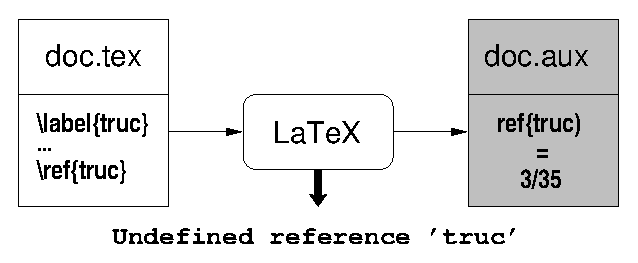
\includegraphics{img/ref1.eps}
    \end{center}
    \caption{使用\dm{.aux}的第一次编译}
    \label{fig:ref1}
  \end{figure}

  因此,此次编译时,会\LaTeX 发送警告,指出标记\dm{truc}未定义。
  \item 我们会进行第二次编译,这次编译会使用辅助文件的内容(如图\ref{fig:ref2}所示)。
  
  \begin{figure}[ht]
    \begin{center}
      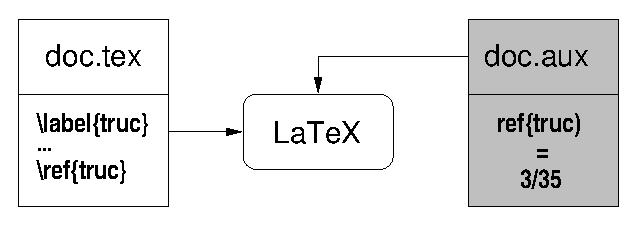
\includegraphics{img/ref2.eps}
    \end{center}
    \caption{使用\dm{.aux}的第二次编译}
    \label{fig:ref2}
  \end{figure}
\end{enumerate}

在以下情况中的引用定义是不正确的。

\begin{enumerate}
  \item 你插入了一个新的标记,并且在插入标记后第一次编译(引用\emph{未被定义})。此时,对于新插入的标记,会得到如下形式的消息:
  
  \begin{dmd}
  Reference 'vlunch' on page 2 undefined on input line 17.
  \end{dmd}

  \item 你在文档中引入的变化无疑会改变页码或对象(图片、方程等)的位置,因此引用会被\emph{错误定义}。在编译结束时,你会看到如下警告:
  
  \begin{dmd}
  Label(s) may have changed.\\
  Rerun to get cross-references right.
  \end{dmd}

  \item 你引用了一个不存在的标记。在这种情况下,再编译八百次也无济于事。
\end{enumerate}

\subsection{与目录的交互}

对于目录,你会发现,其原理与引用是类似的。在文档中插入指令\verb|\tableofcontents|意味着目录将会分两步创建,具体如下。

\begin{enumerate}
  \item 第一轮遍历会收集文档中与\emph{表题}相关的信息,并将其存入文件\codereplace{文件名}\dm{.toc}中(如图\ref{fig:toc1}所示)。
  
  \begin{figure}[ht]
    \begin{center}
      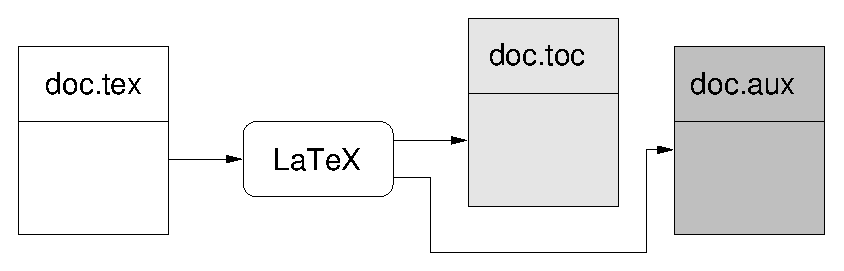
\includegraphics{img/toc1.eps}
    \end{center}
    \caption{使用\dm{.toc}的第一次编译}
    \label{fig:toc1}
  \end{figure}

  \item 第二轮遍历会使最终的文档中包含\codereplace{文件名}\dm{.toc},因此,目录也会被包含(如图\ref{fig:toc2}所示)。
  
  \begin{figure}[ht]
    \begin{center}
      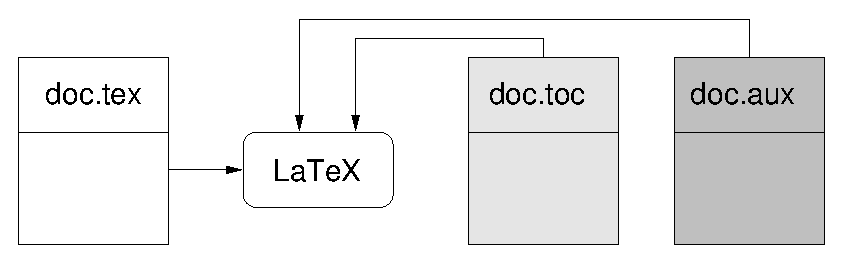
\includegraphics{img/toc2.eps}
    \end{center}
    \caption{使用\dm{.toc}的第二次编译}
    \label{fig:toc2}
  \end{figure}

\end{enumerate}

你可能会遇到这种情况:在写草稿时,文档已经包含了目录指令(\verb|tableofcontents|),而你又添加了新的章节指令。在这种情况下,新的章节只有经过\textbf{两次}编译后才会显示在目录中。

\subsection{一些建议}

要养成为每个文档生成目录的习惯。实际上,\LaTeX 会围绕你的\dm{.tex}文件生成多个文件\jz{
  这还没有涉及参考文献、索引、术语目录等。
}。另外,在起草文档时,不必过于关心目录是否时刻更新——它早晚会更新的!实际上,只有在\textbf{印刷}之前才有必要去确认所有的引用都是正确的。

最后,就像我们在不再能确定目标文件时会时不时运行一下\dm{make clean}指令一样,在看起来一切都运行不正常时,删掉辅助文件\celan{\S B.2}并重新编译是个好习惯。

\section{断字的处理}

\LaTeX 依靠\TeX 对特定的语言来实现不同的断字效果。这种算法在\TeX Book的附录H中有描述,也体现出\TeX 最成功的一面。通过检查文档打断段落的方式,可以识别出文档是不是由\LaTeX 生成的,因为其他很多软件都喜欢以在单词间添加更多空间的方式来处理此类问题。然而,也会有一些\LaTeX 无法正确断字的情况。在这种情况下,\LaTeX 会以以下两种“吓人的”信息之一为你给出警告:

\begin{dmd}
Underfull \backslash hbox (badness 1810) detected at line 33
\end{dmd}

或

\begin{dmd}
Overfull \backslash hbox (14.24376pt too wide) detected at line 41
\end{dmd}

\TeX 在很底层用你的文档生成一系列\emph{字盒}。每个字符都装入合适的字盒,字盒组合成词,再以类似的方式组合成行、成段,然后成页面。

这里以一种简单的方式总结和介绍原理。我们可以简单地理解为,\TeX 在水平模式下操纵\verb|\hbox|来组合单词,在竖直模式下操纵\verb|\vbox|来生成页面。此外,组合这些字盒时,\TeX 如果觉得结果不太美观,就会用以上述两种信息警告你。信息的含义如下。

\begin{itemize}
  \item \verb|Underfull \hbox|表示字盒组合得有些稀疏。通过显示badness的值,\TeX 会告诉你它认为当前行“有多丑”。如果一行文字排列得很完美,该值为0。在最差的情况下,该值为10000.
  \item \verb|Overfull \hbox|表示字盒有些太挤了。\TeX 可以以\dm{pt}为单位显示文字越界深入边缘的长度。
\end{itemize}

如果一个页面过于稀疏,\LaTeX 会以\verb|\vbox|代替\verb|\hbox|显示类似的消息。表\ref{tab:2.4}展示了同一句话的不同疏密程度\yz{
  表中的例句出自法国古典主义戏剧大师高乃依(Pierre Corneille)的戏剧《熙德》(\textit{Le Cid}),意为“哦,愤怒!哦,绝望!哦,宿敌!”。
}排列效果。

\newcommand{\phrase}[1]{\noindent\makebox[\width +
#1][s]{%
  Ô rage ! ô désespoir ! ô vieillesse ennemie !}\par}
\begin{table}[ht] 
\begin{center}
  % \addtolength{\extrarowheight}{4pt} 
  \begin{tabular}{|l|c|}
    \hline
    效果 & 评价 \\
    \hline
    % \typeout{UNDERFULL HBOX AUTORISE}%
    \phrase{1.0cm}  & 稀疏\\
    \phrase{0.75cm} & 稀疏\\
    \phrase{0.45cm} & 稀疏\\
    \hline
    % \typeout{UNDERFULL HBOX AUTORISE}%
    \phrase{0cm}    & 理想 \\ 
    \hline
    \phrase{-0.1cm} & 过密\\
    \phrase{-0.2cm} & 过密\\
    \phrase{-0.25cm} & 过密\\
    \hline
  \end{tabular}
  \caption{横向的不同疏密排列}
  \label{tab:2.4}
\end{center} 
\end{table}

\begin{ii}
  \makebox[\width+2pt][s]{可以在文档选项中启用\dm{draft},来使在出现\dm{Overfull \backslash hbox}问题的位置的侧栏显示一个黑色的\char"258C}
  方块,就像本段的侧栏一样。这个选项可以帮助快速定位导致问题的行。
\end{ii}

\subsection{控制断字}

对于以下情况,\LaTeX 的断字处理可能遇到困难。

\begin{itemize}
  \item 它不能识别需要打断的词——这是个极端情况。
  \item 不能打断的对象占据了需要打断的位置,例如\verb+\verb|...|+或方程类型的对象。
\end{itemize}

这里提供以下几个控制断字的方法。

\begin{exclamation}
如果以下方法都不能使你满意(如果你的句子中包含太多\TeX 不能打断的对象,就会产生这种情况),就只能想办法更换表达方式来规避问题了。
\end{exclamation}

\subsubsection{引导断字}

我们可以通过在必要的位置插入指令\verb|\-|来指出可以断字的位置,从而帮助\LaTeX 实现断字。例如,如果\LaTeX 不能成功地打断“nonmaiçavapamieu”\yz{
  作者的生造词,形似句子“Non, mais ça ne va pas mieux.”,意为“不,没有变得更好”。
}一词,我们可以输入:

\begin{dmd}
\verb|non\-mai\-ça\-va\-pa\-mieu|
\end{dmd}

如果这个词频繁出现,为了避免反复像上面这样给出指示,可以在文前部分输入指令\linebreak \verb|\hyphenation|:

\begin{dmd}
\verb|\hyphenation{non-mai-ça-va-pa-mieu}|
\end{dmd}

这样就可以告诉\LaTeX 这个生词的断字方式。

\subsubsection{强制断字}

通过输入指令\verb|\linebreak[|\codereplace{数字}\verb|]|,我们可以强制断字,但这样做可能带来灾难性的后果——如果你明白我的意思。参数\codereplace{数字}可以调节指令\verb|\linebreak|。你可以“腼腆”地给出指示——\verb|\linebreak[0]|,或是给出不容置疑的命令——\verb|\linebreak[4]|。

指令\verb|\pagebreak[|\codereplace{数字}\verb|]|可以打断页面。另一方面,还有两个指令可以用来换页:

\begin{itemize}
  \item \verb|\clearpage| 完成当前页面,换页另起。
  \item \verb|\cleardoublepage| 完成当前页面,并在双面模式下从奇数页另起。
\end{itemize}

这两条指令会强制\LaTeX 在布局过程中插入所有浮动的图像。%TODO 所以这句是在说啥???

\begin{ii}
另外一种对某些情况很实用的手动介入方式是将当前页面纵向长度加长,需要调用如下指令:

\begin{dmd}
  \backslash enlargethispage
\end{dmd}

指令需要给出尺寸,且其后需要插入一个空行:

\begin{tabbing}
  \verb|\enlargethispage{10cm}   | \= \leftarrow 针对过短的页面 \\
  ~\\
  \verb|[……一段过长的文字……]|\\
  \verb|\clearpage| \> \leftarrow 明确延长10 cm的页面的结尾
\end{tabbing}
\end{ii}

\subsubsection{防止断字}

有三种方式可以强制\LaTeX 不打断文本。

\begin{enumerate}
  \item 通过\verb|~|插入不可打断的空格。
  \item 通过\verb|\mbox{|\codereplace{单词}\verb|}|将词放入一个字盒中\jz{
    这是因为\TeX \textbf{永远不会}打断字盒。
  }。
  \item 对于防止换行使用指令\verb|\nolinebreak|:
  
  \begin{dmd}
  \backslash nolinebreak[\codereplace{数字}]
  \end{dmd}

  同样,为了防止换页,可以使用如下指令:

  \begin{dmd}
    \backslash nopagebreak[\codereplace{数字}]
  \end{dmd}

  其中\codereplace{数字}与\verb|\linebreak|或\verb|\pagebreak|中的作用一致。

\end{enumerate}

\section{小结}

本章介绍了\LaTeX 的标准功能。你如果专心地阅读至此,应该已经可以创建任何类型的简单文档了(目前还不能处理带有公式和图表的文档)。即使你还不能自由地定制你的文档,你的文档的排版质量也会足够好,不需要你提出很多形而上学的问题,如多大的页边距才“理想”、标题和文字间留出多少空白才“合适”……实际上,\LaTeX 中的默认特性已经足够满足全世界范围内有关印刷的大部分实用性规则。

